\documentclass{article}

\usepackage{graphicx}
\usepackage{tikz}
\usepackage{tikzsymbols}
\usetikzlibrary{calc,patterns,shapes.geometric}
\pagestyle{empty}
\usepackage[margin=0pt]{geometry}
\geometry{papersize={14in,12in}}

\def\centerarc[#1](#2)(#3:#4:#5){\draw[#1] ($(#2)+({#5*cos(#3)},{#5*sin(#3)})$) arc (#3:#4:#5);}

\begin{document}
	\begin{figure}
		\centering
		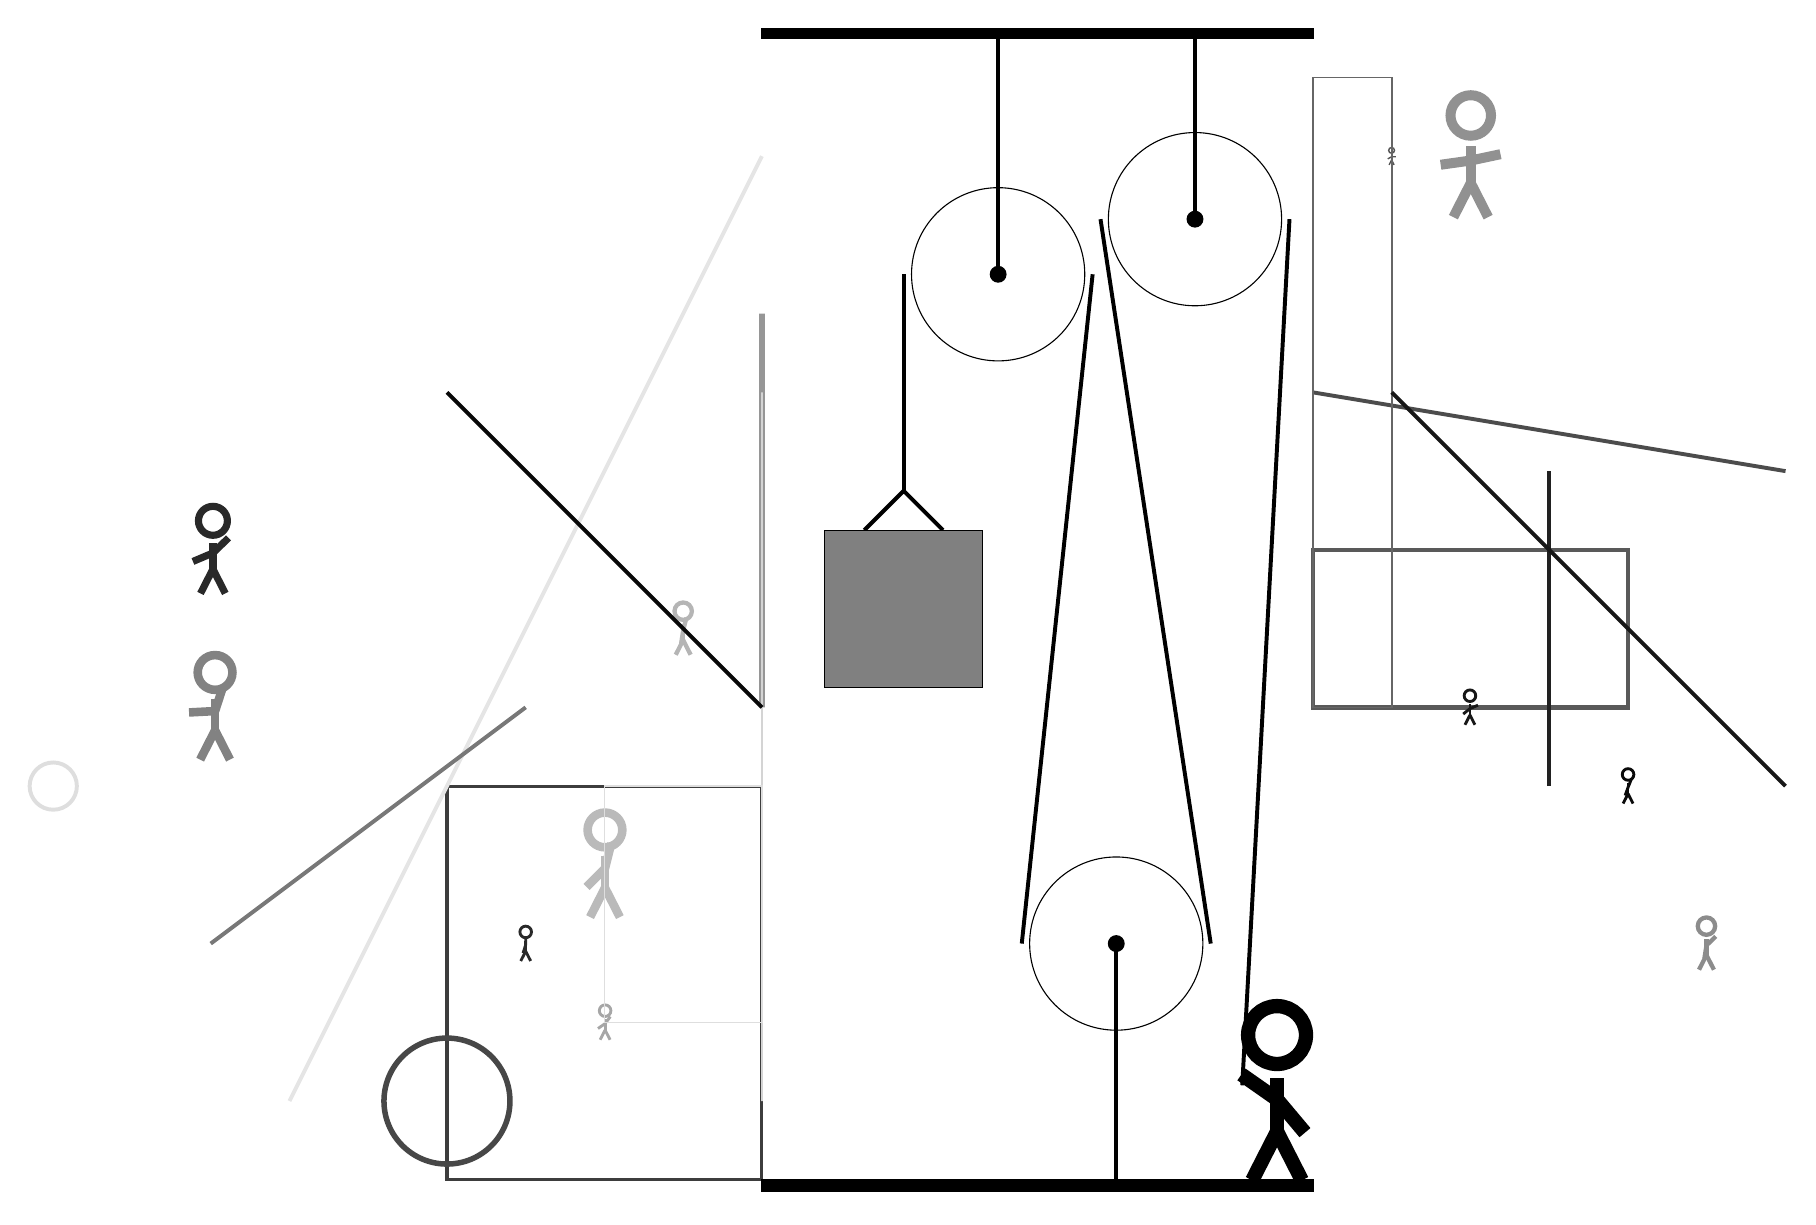
\begin{tikzpicture}
			%%%%% START %%%%%
			
			\draw[fill=black] (-2, 11.5) rectangle (5, 11.625);
			
			\draw (1, 8.5) circle (1.1);
			\draw[fill=black] (1, 8.5) circle (0.1);
			\draw[line width=0.5mm]  (1, 11.5) -- (1, 8.5);
			
			\draw[fill=white](2.5, 0.0) circle (1.1);
			\draw[fill=black] (2.5, 0.0) circle (0.1);
			\draw[line width=0.5mm]  (2.5, -3) -- (2.5, 0.0);
			
			\draw [line width=0.5mm, color=black!13](-11, 2) circle (0.3);
			
			\node[line width=0.7mm, color=black!35] at (-4, -1) {\Strichmaxerl[2][35][53]};
			\draw[line width=0.4mm, color=black!76] (-2, -3) rectangle (-6, 2);
			\draw[line width=0.5mm, color=black!70](5, 7) -- (11, 6);
			\draw[line width=0.6mm, color=black!65] (5, 3) rectangle (9, 5);
			\node[line width=0.3mm, color=black!84] at (-5, 0) {\Strichmaxerl[2][72][89]};
			
			\node[line width=0.2mm, color=black!29] at (-3, 4) {\Strichmaxerl[3][81][76]};
			\draw[line width=0.5mm, color=black!10](-2, 10) -- (-8, -2);
			\node[line width=0.5mm, color=black!96] at (9, 2) {\Strichmaxerl[2][70][68]};
			\node[line width=0.7mm, color=black!45] at (10, 0) {\Strichmaxerl[3][81][44]};
			
			\draw[line width=0.7mm, color=black!41] (-2, 3) rectangle (-2, 8);
			\draw[line width=0.3mm, color=black!17] (-2, -2) rectangle (-2, 7);
			\node[line width=0.2mm, color=black!49] at (-9, 3) {\Strichmaxerl[6][3][72]};
			
			\draw [line width=0.7mm, color=black!72](-6, -2) circle (0.8);
			\node[line width=0.2mm, color=black!43] at (7, 10) {\Strichmaxerl[7][8][12]};
			\node[line width=0.7mm, color=black!27] at (-4, 1) {\Strichmaxerl[6][45][76]};
			
			\draw[line width=0.5mm, color=black!97](-2, 3) -- (-6, 7);
			\draw[line width=0.2mm, color=black!13] (-2, 2) rectangle (-4, -1);
			\node[line width=0.7mm, color=black!84] at (-9, 5) {\Strichmaxerl[5][23][44]};
			\node[line width=0.5mm, color=black!67] at (6, 10) {\Strichmaxerl[1][28][1]};
			\node[line width=0.2mm, color=black!91] at (7, 3) {\Strichmaxerl[2][39][23]};
			
			\draw[line width=0.2mm, color=black!60] (5, 3) rectangle (6, 11);
			\draw[line width=0.5mm, color=black!87](8, 2) -- (8, 6);
			\draw[line width=0.5mm, color=black!53](-5, 3) -- (-9, 0);
			\draw[line width=0.5mm, color=black!91](6, 7) -- (11, 2);
			
			\draw[fill=white](3.5, 9.2) circle (1.1);
			\draw[fill=black] (3.5, 9.2) circle (0.1);
			\draw[line width=0.5mm] (3.5, 11.5) -- (3.5, 9.2);
			
			\draw[line width=0.5mm] (-0.7, 5.25) -- (-0.2, 5.75) -- (0.3, 5.25);
			\draw[fill=black!50] (-1.2, 5.25) rectangle (0.8, 3.25);
			
			\draw[line width=0.5mm] (-0.2, 8.5) -- (-0.2, 5.75);
			\centerarc[line width=0.5mm](1, 8.5)(0:180:1.2000000000000002);
			\draw[line width=0.5mm](2.2, 8.5) -- (1.3, 0.0);
			\centerarc[line width=0.5mm](2.5, 0.0)(180:360:1.2000000000000002);
			\draw[line width=0.5mm](3.7, 0.0) -- (2.3, 9.2);
			\centerarc[line width=0.5mm](3.5, 9.2)(0:180:1.2000000000000002);
			\draw[line width=0.5mm](4.7, 9.2) -- (4.1, -1.8);
			
			\node at (4.5, -1.9) {\Strichmaxerl[10][-35][-50]};
			
			\draw[fill=black] (-2, -3) rectangle (5, -3.15);
			
			%%%%% END %%%%%
		\end{tikzpicture}
	\end{figure}	
\end{document}